\chapter{Condicionales y recursión}

\section{El operador residuo}

\index{operador residuo} \index{operador!residuo}

El \textbf{operador residuo} trabaja con enteros (y expresiones enteras)
calculando el residuo del primer operando cuando se divide por el
segundo. En Python este operador es un signo porcentaje (\texttt{\%}).
La sintaxis es la misma que para los otros operadores:

\begin{pyconcode}
>>> cociente = 7 // 3
>>> print(cociente)
2
>>> residuo = 7 % 3
>>> print(residuo)
1
\end{pyconcode}

Así que 7 dividido por 3 da 2 con residuo 1.

El operador residuo resulta ser sorprendentemente útil. Por ejemplo,
usted puede chequear si un número es divisible por otro si \texttt{x\%y}
es cero, entonces \texttt{x} es divisible por \texttt{y}.

Usted también puede extraer el dígito o dígitos más a la derecha de
un número. Por ejemplo, \texttt{x \% 10} entrega el dígito más a la
derecha de \texttt{x} (en base 10). Igualmente, \texttt{x \% 100}
entrega los dos últimos dígitos.

\section{Expresiones booleanas}

\index{expresión Booleana} \index{expresión!booleana} \index{operador lógico}
\index{operador!lógico}

El tipo que Python provee para almacenar valores de verdad (cierto
o falso) se denomina bool por el matemático británico George Bool.
Él creó el Álgebra Booleana, que es la base para la aritmética que
se usa en los computadores modernos.

Sólo hay dos valores booleanos: True (cierto) y False (falso). Las
mayúsculas importan, ya que true y false no son valores booleanos.

El operador \texttt{==} compara dos valores y produce una expresión
booleana:

\begin{pyconcode}
>>> 5 == 5
True
>>> 5 == 6
False
\end{pyconcode}
 En la primera sentencia, los dos operandos son iguales, así que la
expresión evalúa a True (cierto); en la segunda sentencia, 5 no es
igual a 6, así que obtenemos False (falso).

El operador \texttt{==} es uno de los \textbf{operadores de comparación};
los otros son:
\begin{pyconcode}
      x != y               # x no es igual y
      x > y                # x es mayor que y
      x < y                # x es menor que y
      x >= y               # x es mayor o igual a y
      x <= y               # x es menor o igual a y
\end{pyconcode}

Aunque estas operaciones probablemente son familiares para usted,
los símbolos en Python difieren de los matemáticos. Un error común
consiste en usar un solo signo igual (\texttt{=}) en lugar en un doble
signo igual (\texttt{==}). Recuerde que \texttt{=} es el operador
para la asignación y que \texttt{==} es el operador para comparación.
Tenga en cuenta que no existen los signos \texttt{=\textless{}} o
\texttt{=\textgreater{}}.

\section{Operadores lógicos}

\index{operadores lógicos} \index{operador!lógicos}

Hay tres \textbf{operadores lógicos}: \texttt{and}, \texttt{or} y
\texttt{not}. La semántica (el significado) de ellos es similar a
su significado en inglés. Por ejemplo, \texttt{x\textgreater{}0 and
x\textless{}10} es cierto, sólo si \texttt{x} es mayor a cero {\em
y} menor que 10.

\texttt{n\%2 == 0 or n\%3 == 0} es cierto si {\em alguna} de las
condiciones es cierta, esto es, si el número es divisible por 2 {\em
o} por 3.

Finalmente, el operador \texttt{not} niega una expresión booleana,
así que \texttt{not(x\textgreater{}y)} es cierta si \texttt{(x\textgreater{}y)}
es falsa, esto es, si \texttt{x} es menor o igual a \texttt{y}.

Formalmente, los operandos de los operadores lógicos deben ser expresiones
booleanas, pero Python no es muy formal. Cualquier número diferente
de cero se interpreta como ``cierto.''
\begin{pyconcode}
>>>  x = 5
>>>  x and 1
1
>>>  y = 0
>>>  y and 1
0
\end{pyconcode}

En general, esto no se considera un buen estilo de programación. Si
usted desea comparar un valor con cero, procure codificarlo explícitamente.

\section{Ejecución condicional}

\label{alternative execution} \index{ramificación condicional}
\index{ejecución condicional}

A fin de escribir programas útiles, casi siempre necesitamos la capacidad
de chequear condiciones y cambiar el comportamiento del programa en
consecuencia. Las \textbf{sentencias condicionales} nos dan este poder.
La más simple es la sentencia \texttt{if}: 
\begin{pythoncode}
if x > 0:
  print("x es positivo")
\end{pythoncode}

La expresión después de la sentencia \texttt{if} se denomina la \textbf{condición}.
Si es cierta, la sentencia de abajo se ejecuta. Si no lo es, no pasa
nada.

\index{sentencia compuesta} \index{sentencia compuesta!cabecera}
\index{sentencia compuesta!cuerpo} \index{sentencia compuesta!bloque de sentencias}
\index{sentencia!compuesta}

Como otras sentencias compuestas, la sentencia \texttt{if} comprende
una cabecera y un bloque de sentencias:
\begin{pythoncode}
CABECERA:
  PRIMERA SENTENCIA
  ...
  ULTIMA SENTENCIA
\end{pythoncode}
La cabecera comienza en una nueva línea y termina con dos puntos seguidos
(:). Las sentencias sangradas o indentadas que vienen a continuación
se denominan el \textbf{bloque}. La primera sentencia sin sangrar
marca el fin del bloque. Un bloque de sentencias dentro de una sentencia
compuesta también se denomina el \textbf{cuerpo} de la sentencia.

\index{bloque} \index{sentencia!bloque} \index{cuerpo}

No hay límite en el número de sentencias que pueden aparecer en el
cuerpo de una sentencia, pero siempre tiene que haber, al menos, una.
Ocasionalmente, es útil tener un cuerpo sin sentencias (como un hueco
para código que aún no se ha escrito). En ese caso se puede usar la
sentencia \texttt{pass}, que no hace nada.

\index{sentencia pass} \index{sentencia!pass}

\section{Ejecución alternativa}

\label{alternative execution2}

Una segunda forma de sentencia \texttt{if} es la ejecución alternativa
en la que hay dos posibilidades y la condición determina cual de ellas
se ejecuta. La sintaxis luce así:
\begin{pythoncode}
if x%2 == 0:
  print(x, "es par")
else:
  print(x, "es impar")
\end{pythoncode}

Si el residuo de dividir \texttt{x} por 2 es 0, entonces sabemos que
\texttt{x} es par, y el programa despliega un mensaje anunciando esto.
Si la condición es falsa, la segunda sentencia se ejecuta. Como la
condición, que es una expresión booleana, debe ser cierta o falsa,
exactamente una de las alternativas se va a ejecutar. Estas alternativas
se denominan \textbf{ramas}, porque, de hecho, son ramas en el flujo
de ejecución.

\index{rama}

Yéndonos ``por las ramas'', si usted necesita chequear la paridad
(si un número es par o impar) a menudo, se podría ``envolver'' el
código anterior en una función:
\begin{pythoncode}
def imprimirParidad(x):
  if x%2 == 0:
    print(x, "es par")
  else:
    print(x, "es impar")
\end{pythoncode}

Para cualquier valor de \texttt{x}, \texttt{imprimirParidad} despliega
un mensaje apropiado. Cuando se llama la función, se le puede pasar
cualquier expresión entera como argumento.
\begin{pythoncode}
>>> imprimirParidad(17)
>>> imprimirParidad(y+1)
\end{pythoncode}

\section{Condicionales encadenados}

\index{condicional encadenados} \index{condicional!encadenados}

Algunas veces hay más de dos posibilidades y necesitamos más de dos
ramas. Una forma de expresar un cálculo así es un \textbf{condicional
encadenado}:

\begin{pythoncode}
if x < y:
  print(x, "es menor que", y)
elif x > y:
  print(x, "es mayor que", y)
else:
  print(x, "y", y, "son iguales")
\end{pythoncode}

\texttt{elif} es una abreviatura de ``else if.'' De nuevo, exactamente
una de las ramas se ejecutará. No hay límite en el número de sentencias
\texttt{elif}, pero la última rama tiene que ser una sentencia \texttt{else}:
\begin{pythoncode}
if eleccion == 'A':
  funcionA()
elif eleccion == 'B':
  funcionB()
elif eleccion == 'C':
  funcionC()
else:
  print("Eleccion incorrecta.")
\end{pythoncode}

Cada condición se chequea en orden. Si la primera es falsa, se chequea
la siguiente, y así sucesivamente. Si una de ellas es cierta, se ejecuta
la rama correspondiente y la sentencia termina. Si hay más de una
condición cierta, sólo la primera rama que evalúa a cierto se ejecuta.

\section{Condicionales anidados}

Un condicional también se puede anidar dentro de otro. La tricotomía
anterior se puede escribir así:

\begin{pythoncode}
if x == y:
  print(x, "y", y, "son iguales")
else:
  if x < y:
    print(x, "es menor que", y)
  else:
    print(x, "es mayor que", y)
\end{pythoncode}
 El condicional externo contiene dos ramas: la primera contiene una
sentencia de salida sencilla, la segunda contiene otra sentencia \texttt{if},
que tiene dos ramas propias. Esas dos ramas son sentencias de impresión,
aunque también podrían ser sentencias condicionales.

Aunque la indentación o sangrado de las sentencias sugiere la estructura,
los condicionales anidados rápidamente se hacen difíciles de leer.
En general, es una buena idea evitarlos cada vez que se pueda.

Los operadores lógicos proporcionan formas de simplificar las sentencias
condicionales anidadas. Por ejemplo, podemos reescribir el siguiente
código usando un solo condicional:
\begin{pythoncode}
if 0 < x:
  if x < 10:
    print("x es un digito positivo.")
\end{pythoncode}

La sentencia \texttt{print} se ejecuta solamente si el flujo de ejecución
ha pasado las dos condiciones, así que podemos usar el operador \texttt{and}:
\begin{pythoncode}
if 0 < x and x < 10:
  print("x es un digito positivo.")
\end{pythoncode}

Esta clase de condiciones es muy común, por esta razón Python proporciona
una sintaxis alternativa que es similar a la notación matemática:
\begin{pythoncode}
if 0 < x < 10:
  print("x es un digito positivo")
\end{pythoncode}

Desde el punto de vista semántico ésta condición es la misma que la
expresión compuesta y que el condicional anidado.

\section{La sentencia \texttt{return} }

\index{sentencia return} \index{sentencia!return}

La sentencia \texttt{return} permite terminar la ejecución de una
función antes de llegar al final. Una razón para usarla es reaccionar
a una condición de error:

\begin{pythoncode}
import math

def imprimirLogaritmo(x):
  if x <= 0:
    print("Numeros positivos solamente. Por favor")
    return

  result = math.log(x)
  print("El logaritmo de ",  x ," es ", result)
\end{pythoncode}
 La función \texttt{imprimirLogaritmo} toma un parámetro denominado
\texttt{x}. Lo primero que hace es chequear si \texttt{x} es menor
o igual a 0, caso en el que despliega un mensaje de error y luego
usa a \texttt{return} para salir de la función. El flujo de ejecución
inmediatamente retorna al punto donde se había llamado la función,
y las líneas restantes de la función no se ejecutan.

Recuerde que para usar una función del módulo matemático (math) hay
que importarlo previamente.

\section{Recursión}

\label{recursion} \index{recursión}

Hemos mencionado que es legal que una función llame a otra, y usted
ha visto varios ejemplos así. Hemos olvidado mencionar el hecho de
que una función también puede llamarse a sí misma. Al principio no
parece algo útil, pero resulta ser una de las capacidades más interesantes
y mágicas que un programa puede tener. Por ejemplo, observe la siguiente
función:

\begin{pythoncode}
def conteo(n):
  if n == 0:
    print("Despegue!")
  else:
    print(n)
    conteo(n-1)
\end{pythoncode}

\texttt{conteo} espera que el parámetro \texttt{n} sea un número entero
positivo. Si \texttt{n} es 0, despliega la cadena, ``Despegue!''.
Si no lo es, despliega \texttt{n} y luego llama a la función llamada
\texttt{conteo}—ella misma—pasando a \texttt{n-1} como argumento.

Analicemos lo que sucede si llamamos a esta función así:
\begin{pyconcode}
>>> conteo(3)
\end{pyconcode}

La ejecución de \texttt{conteo} comienza con \texttt{n=3}, y como
\texttt{n} no es 0, despliega el valor 3, y se llama a sí misma ...
\begin{quote}
La ejecución de \texttt{conteo} comienza con \texttt{n=2}, y como
\texttt{n} no es 0, despliega el valor 2, y se llama a si misma ...

\begin{quote}
La ejecución de \texttt{conteo} comienza con \texttt{n=1}, y como
\texttt{n} no es 0, despliega el valor 1, y se llama a sí misma ...

\begin{quote}
La ejecución de \texttt{conteo} comienza con \texttt{n=0}, y como
\texttt{n} es 0, despliega la cadena ``Despegue!'' y retorna (finaliza). 
\end{quote}
El \texttt{conteo} que recibió \texttt{n=1} retorna. 
\end{quote}
El \texttt{conteo} que recibió \texttt{n=2} retorna. 
\end{quote}
El \texttt{conteo} que recibió \texttt{n=3} retorna.

Y el flujo de ejecución regresa a \texttt{\_\_main\_\_} (vaya viaje!).
Así que, la salida total luce así:
\begin{pythoncode}
3
2
1
Despegue!
\end{pythoncode}
Como otro ejemplo, utilizaremos nuevamente las funciones \texttt{nuevaLinea}
y \texttt{tresLineas}:

\begin{pythoncode}
def nuevalinea():
  print()

def tresLineas():
  nuevaLinea()
  nuevaLinea()
  nuevaLinea()
\end{pythoncode}

Este trabajo no sería de mucha ayuda si quisiéramos desplegar 2 líneas
o 106. Una mejor alternativa sería:

\begin{pythoncode}
def nLineas(n):
  if n > 0:
    print()
    nLineas(n-1)
\end{pythoncode}
 Esta función es similar a \texttt{conteo}; en tanto \texttt{n} sea
mayor a 0, despliega una nueva línea y luego se llama a sí misma para
desplegar \texttt{n-1} líneas adicionales. Así, el número total de
nuevas líneas es \texttt{1 + (n - 1)} que, si usted verifica con álgebra,
resulta ser \texttt{n}.

El proceso por el cual una función se llama a sí misma es la \textbf{recursión},
y se dice que estas funciones son recursivas.

\index{recursión} \index{función!recursiva}

\section{Diagramas de pila para funciones recursivas}

\index{diagrama de pila} \index{marco de función} \index{marco}

En la Sección~\ref{stackdiagram}, usamos un diagrama de pila para
representar el estado de un programa durante un llamado de función.
La misma clase de diagrama puede ayudarnos a interpretar una función
recursiva.

Cada vez que una función se llama, Python crea un nuevo marco de función
que contiene los parámetros y variables locales de ésta. Para una
función recursiva, puede existir más de un marco en la pila al mismo
tiempo.

Este es el diagrama de pila para \texttt{conteo} llamado con \texttt{n
= 3}:

\beforefig \centerline{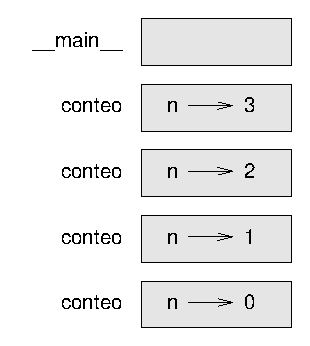
\includegraphics{illustrations/stack2}}
\afterfig

Como siempre, el tope de la pila es el marco para \texttt{\_\_main\_\_}.
Está vacío porque no creamos ninguna variable en \texttt{\_\_main\_\_}
ni le pasamos parámetros.

Los cuatro marcos de \texttt{conteo} tienen diferentes valores para
el parámetro \texttt{n}. El fondo de la pila, donde \texttt{n=0},
se denomina el \textbf{caso base }. Como no hace una llamada recursiva,
no hay mas marcos.

\index{case base} \index{recursión!caso base}

\section{Recursión infinita}

\index{recursión infinita} \index{recursión!infinita} \index{error de tiempo de ejecución}
\index{error!de tiempo de ejecución} \index{trazado inverso}

Si una función recursiva nunca alcanza un caso base va a hacer llamados
recursivos por siempre y el programa nunca termina. Esto se conoce
como \textbf{recursión infinita}, y, generalmente, no se considera
una buena idea. Aquí hay un programa minimalista con recursión infinita:

\begin{pythoncode}
def recurrir():
  recurrir()
\end{pythoncode}
 En la mayoría de ambientes de programación un programa con recursión
infinita no corre realmente para siempre. Python reporta un mensaje
de error cuando alcanza la máxima profundidad de recursión:
\begin{pythoncode}
  File "<stdin>", line 2, in recurrir
  (98 repeticiones omitidas)
  File "<stdin>", line 2, in recurrir
RuntimeError: Maximum recursion depth exceeded
\end{pythoncode}
Este trazado inverso es un poco más grande que el que vimos en el
capítulo anterior. Cuando se presenta el error, ¡hay más de 100 marcos
de \texttt{recurrir} en la pila!.

\section{Entrada por el teclado}

Los programas que hemos escrito son un poco toscos ya que no aceptan
entrada de un usuario. Sólo hacen la misma operación todo el tiempo.

Python proporciona funciones primitivas que obtienen entrada desde
el teclado. La más sencilla se llama \texttt{input}. Cuando esta
función se llama el programa se detiene y espera a que el usuario
digite algo. Cuando el usuario digita la tecla Enter o Intro, el programa
retoma la ejecución y \texttt{input} retorna lo que el usuario
digitó como una cadena (\texttt{string}):

\begin{pyconcode}
>>> entrada = input()
Que esta esperando?
>>> print(entrada)
Que esta esperando?
\end{pyconcode}

Antes de llamar a \texttt{input} es una muy buena idea desplegar
un mensaje diciéndole al usuario qué digitar. Este mensaje se denomina
indicador de entrada (\textbf{prompt} en inglés). Podemos dar un argumento
prompt a \texttt{input}:

\index{prompt}

\begin{pyconcode}
>>> nombre = input("Cual es tu nombre? ")
Cual es tu nombre? Arturo, Rey de los Bretones!
>>> print(nombre)
Arturo, Rey de los Bretones!
\end{pyconcode}

En Python 3 la función \texttt{input} devuelve cadenas de texto. Si esperamos 
que la respuesta sea un entero, podemos usar la función \texttt{int} para intentar
convertir esa cadena ingresada en un número entero:

\begin{pythoncode}
prompt = "Cual es la velocidad de una golondrina sin carga?\n"
velocidad = int(input(prompt))
\end{pythoncode}

Si el usuario digita una cadena de dígitos, éstos se convierten a
un entero que se asigna a \texttt{velocidad}. Desafortunadamente,
si el usuario digita una entrada que no representa un dígito, el 
programa fallará.

\begin{pyconcode}
>>> prompt = "Cual es la velocidad una golondrina sin carga?\n"
>>> velocidad = int(input(prompt))
Que quiere decir, una golondria Africana o Europea?
Traceback (most recent call last):
File "<stdin>", line 1, in <module>
ValueError: invalid literal for int() with base 10: 'Que quiere decir, una golondria Africana o Europea?'
\end{pyconcode}

\section{Glosario}
\begin{description}
\item [{Operador residuo:}] operador que se denota con un signo porcentaje
(\texttt{\%}), y trabaja sobre enteros produciendo el residuo de un
número al dividirlo por otro.
\item [{Expresión booleana:}] expresión cierta o falsa.
\item [{Operador de comparación:}] uno de los operadores que compara
dos valores: \texttt{==}, \texttt{!=}, \texttt{\textgreater{}}, \texttt{\textless{}},
\texttt{\textgreater{}=}, y \texttt{\textless{}=}.
\item [{Operador lógico:}] uno de los operadores que combina expresiones
booleanas: \texttt{and}, \texttt{or}, y \texttt{not}.
\item [{Sentencia condicional:}] sentencia que controla el flujo de ejecución
dependiendo de alguna condición.
\item [{Condición:}] la expresión booleana en una sentencia condicional
que determina que rama se ejecuta.
\item [{Sentencia compuesta:}] es la sentencia que comprende una cabecera
y un cuerpo. La cabecera termina con dos puntos seguidos (:). El cuerpo
se sangra o indenta con respecto a la cabecera.
\item [{Bloque:}] grupo de sentencias consecutivas con la misma indentación.
\item [{Cuerpo:}] el bloque, en una sentencia compuesta, que va después
de la cabecera.
\item [{Anidamiento:}] situación en la que hay una estructura dentro de
otra, tal como una sentencia condicional dentro de una rama de otra
sentencia condicional.
\item [{Recursión:}] es el proceso de llamar la función que se está ejecutando
actualmente.
\item [{Caso base:}] corresponde a una rama de la sentencia condicional
dentro de una función recursiva, que no hace un llamado recursivo.
\item [{Recursión infinita:}] función que se llama a sí misma recursivamente
sin alcanzar nunca el caso base. En Python una recursión infinita
eventualmente causa un error en tiempo de ejecución.
\item [{Prompt (indicador de entrada):}] una pista visual que le indica
al usuario que digite alguna información.

\index{operador residuo} \index{expresión booleana} \index{expresión!booleana}
\index{sentencia condicional} \index{sentencia!condicional} \index{condición}
\index{sentencia compuesta} \index{rama} \index{cuerpo} \index{bloque}
\index{anidamiento} \index{recursión} \index{caso base} \index{recursión infinita}
\index{prompt}
\end{description}

\section{Ejercicios}
\begin{enumerate}
\item Evalúe la expresión \verb+7 % 0+. Explique lo que ocurre.
\item Envuelva el código que viene a continuación en una función llamada
\verb+comparar(x, y)+. Llame a la función comparar tres veces: una
en la que el primer argumento sea menor que el segundo, otra en la
que aquel sea mayor que éste, y una tercera en la que los argumentos
sean iguales. 
\begin{pythoncode}
 if x < y:
    print(x, "es menor que", y)
 elif x > y:
    print(x, "es mayor que", y)
 else:
    print(x, "y", y, "son iguales")
\end{pythoncode}
\item Copie este programa en un archivo llamado tabladeverdad.py: 
\begin{pythoncode}
def tabladeverdad(expresion):
    print(" p      q      %s"  % expresion)
    longitud = len( " p      q      %s"  % expresion)
    print(longitud*"=")

    for p in True, False:
        for q in True, False:
            print("%-7s %-7s %-7s" % (p, q, eval(expresion)))
\end{pythoncode}

Pruébelo con el llamado \verb+tabladeverdad("p or q")+. Ahora ejecútelo
con las siguientes expresiones: 
\begin{enumerate}
\item \texttt{\char`\"{}not(p or q)\char`\"{}} 
\item \texttt{\char`\"{}p and q\char`\"{}} 
\item \texttt{\char`\"{}not(p and q)\char`\"{}} 
\item \texttt{\char`\"{}not(p) or not(q)\char`\"{}} 
\item \texttt{\char`\"{}not(p) and not(q)\char`\"{} }
\end{enumerate}
¿Cuales de estas expresiones tienen el mismo valor de verdad (son
lógicamente equivalentes)?
\end{enumerate}